\documentclass{fenicscourse}

\begin{document}

%\fenicslecture{Overview}{Martin Sandve Aln{\ae}s}
%\fenicslectureoverview{Martin Sandve Aln{\ae}s}{Lund, June 9-10 2015}
\fenicslectureoverview{Anders Logg}{Beijing, August 5--7 2015}

\begin{frame}
  \frametitle{Course outline}

  % Course plan
  %
  % Wed 2015-08-05 14.00-14.45 (45 min)
  %                14.55-15.40 (45 min)
  %                15.50-16.35 (45 min)
  %                16.45-17.30 (45 min)
  % Thu 2015-08-06 14.00-14.45 (45 min)
  %                14.55-15.40 (45 min)
  %                15.50-16.35 (45 min)
  %                16.45-17.30 (45 min)
  % Fri 2015-08-07 14.00-14.45 (45 min)
  %                14.55-15.40 (45 min)
  %                15.50-16.35 (45 min)
  %                16.45-17.30 (45 min)
  %
  % Total: 12 hours (9 hours)
  %
  % Monday
  %
  %   ---  This overview                30 min
  %   L01  Installation of FEniCS       15 min  (if required also do L00)
  %   L02  Static linear PDEs           45 min lecture
  %   L02  Static linear PDEs           45 min challenge
  %   L04  Time-dependent PDEs          45 min lecture
  %
  % Tuesday
  %
  %   L06  Static hyperelasticity       45 min lecture
  %   L06  Static hyperelasticity       45 min challenge
  %   L07  Dynamic hyperelasticity      45 min lecture
  %   L07  Dynamic hyperelasticity      45 min challenge
  %
  % Wednesday
  %
  %   L08  The Stokes problem            45 min lecture
  %   L08  The Stokes problem            45 min challenge
  %   L09  Incompressible Navier-Stokes  45 min lecture
  %   L09  Incompressible Navier-Stokes  45 min challenge
  %
  % Friday
  %
  %   L10  Discontinuous Galerkin methods for elliptic equations
  %   L11  A posteriori error estimates and adaptivity
  %
  % Modifications on site: students not used to programming and
  % difficultites to understand instruction (English).
  %
  % - Move L04 to Tuesday (needed more time for challenge)
  % - Skip L07 (new material instead)
  % - Start day 2 with live demo / tutorial of nonlinear Poisson
  % - Use BoxMesh instead of LEGO for L06 since no internet access

  % Note to lecturers: use \textcolor{grey}{Lecture title} to mark
  % lectures that are not included in a course

  \begin{enumerate}
  \item[$\star$]
    Overview and Introduction (UPDATED!)
  \item[\textcolor{black}{\it Wed} L01]
    Installation of FEniCS
  \item[L02]
    Static linear PDEs
  \item[L04]
    \textcolor{grey}{Time-dependent PDEs}
    \bigskip
  \item[\textcolor{black}{\it Thu} ***]
    Live demonstration: nonlinear Poisson
  \item[L04]
    Time-dependent PDEs
  \item[L06]
    Static hyperelasticity
  \item[L07]
    \textcolor{grey}{Dynamic hyperelasticity}
    \bigskip
  \item[\textcolor{black}{\it Fri} L08]
    The Stokes problem
  \item[L09]
    Incompressible Navier--Stokes
  \end{enumerate}

  \normalsize

\end{frame}

\begin{frame}
  \frametitle{Full list of FEniCS lectures}

  % Note to lecturers: use \textcolor{grey}{Lecture title} to mark
  % lectures that are not included in a course

  \scriptsize
  \begin{enumerate}
  \item[$\star$]
    Overview and Introduction
  \item[L00]
    \textcolor{grey}{Introduction to FEM}
  \item[L01]
    Installation of FEniCS
  \item[L02]
    Static linear PDEs
  \item[L03]
    \textcolor{grey}{Static nonlinear PDEs}
  \item[L04]
    Time-dependent PDEs
  \item[L05]
    \textcolor{grey}{Happy hacking: Tools, tips and coding practices}
  \item[L06]
    Static hyperelasticity
  \item[L07]
    Dynamic hyperelasticity
  \item[L08]
    The Stokes problem
  \item[L09]
    Incompressible Navier--Stokes
  \item[L10]
    \textcolor{grey}{Discontinuous Galerkin methods for elliptic equations}
  \item[L11]
    \textcolor{grey}{A posteriori error estimates and adaptivity}
  \item[L12]
    \textcolor{grey}{Computing sensitivities}
  \item[L13]
    \textcolor{grey}{Introduction to dolfin-adjoint}
  \item[L14]
    \textcolor{grey}{From sensitivities to optimisation}
  \item[L14]
    \textcolor{grey}{One-shot optimisation}
  \item[L16]
    \textcolor{grey}{Optimal control of the Navier-Stokes equations}
  \end{enumerate}

  \normalsize

  {\footnotesize All lectures can be downloaded from
    \url{http://fenicsproject.org/pub/course/}}

\end{frame}

% The quickest FEniCS intro
\begin{frame}
\medskip

\includegraphics[width=0.99\textwidth]{png/fenics_banner.png}
\begin{columns}[c]
\begin{column}{0.4\textwidth}
\bf{The FEniCS Project is a collection of open-source software
  components aimed at the numerical solution of partial differential
  equations using finite element methods}
\end{column}
\begin{column}{0.7\textwidth}
  \begin{block}{Key distinguishing features}
  \begin{itemize}
  \item
    FEniCS (Python/C++) code is quick to write and easy to read
  \item
    `Any' finite element formulation of 'any' partial differential
    equation can be coded
  \item
    Automated code generation is heavily used under the hood to
    create efficient, specialized, low-level code
  \item
    Performance -- implicit problems with over $12\, 000\, 000\, 000$
    degrees of freedom can be solved in a couple of minutes
  \end{itemize}
  \end{block}
\end{column}
\end{columns}
  \begin{center}
    \colemph{\url{http://fenicsproject.org/}}
  \end{center}
\end{frame}

\begin{frame}
\frametitle{FEniCS has been used for a wide range of
  equations and applications}

{\tiny Reaction-diffusion equations; Stokes with or without nonlinear
  viscosity; compressible and incompressible Navier--Stokes; RANS
  turbulence models; shallow water equations; Bidomain equations;
  nonlinear and linear elasticity; nonlinear and linear
  viscoelasticity; Schr\"odinger; Biot's equations for porous media,
  fracture mechanics, electromagnetism, liquid crystals including
  liquid crystal elastomers, combustion, ... and coupled systems of
  the above, ...}

\begin{center}
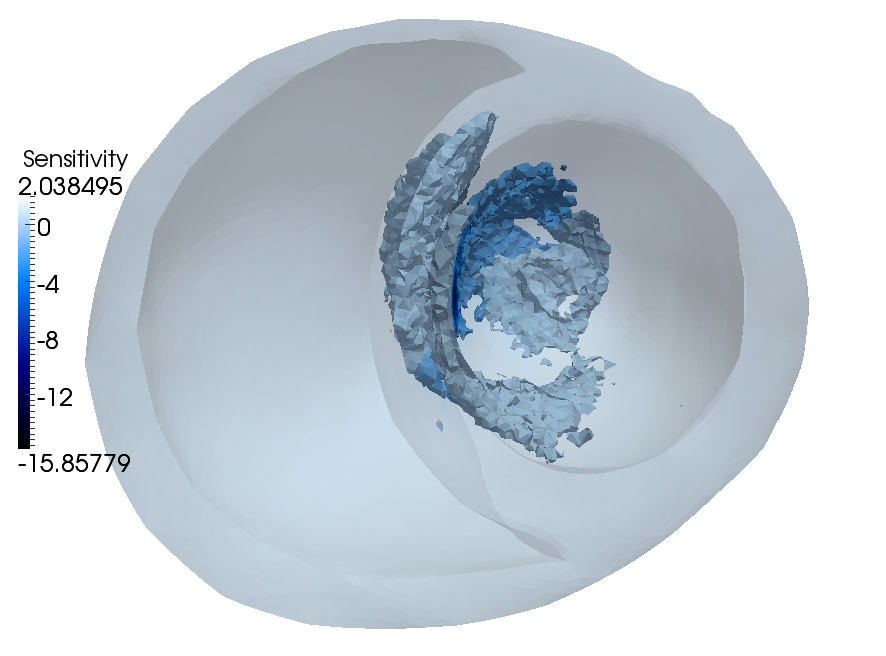
\includegraphics[width=0.24\textwidth]{png/g_el_plusx.png}
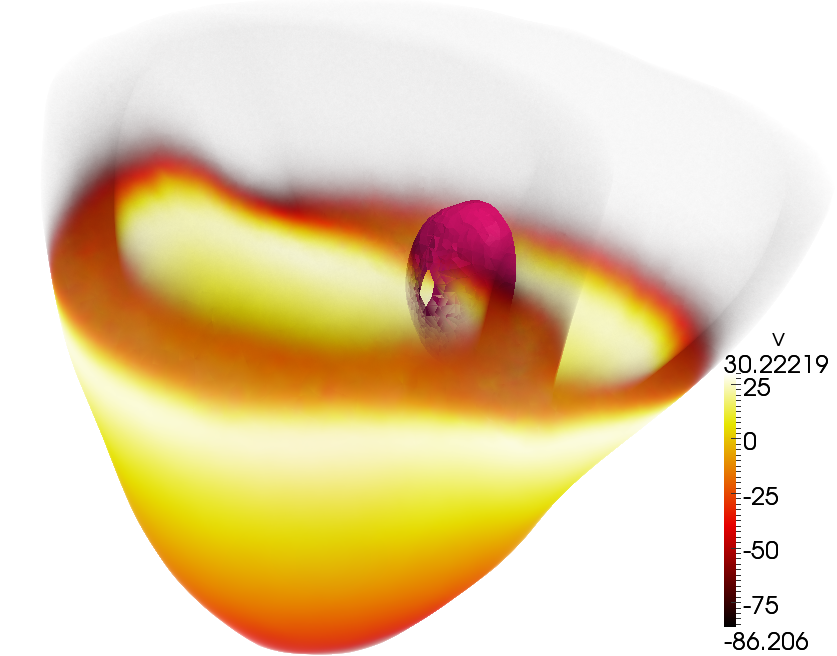
\includegraphics[width=0.24\textwidth]{png/unhealthy_v_at_T200.png}
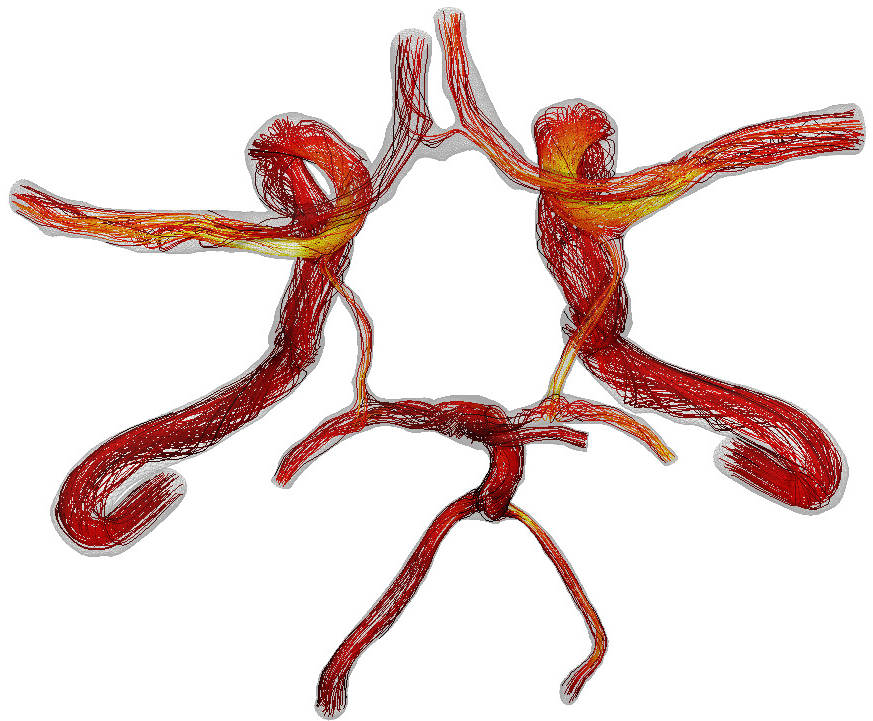
\includegraphics[width=0.24\textwidth]{png/circle_of_willis_simulation.png}
\end{center}

{\tiny for simulating blood flow, computing calcium release in cardic
  tissue, computing the cardiac potential in the heart, simulating
  mantle convection, simulating melting ice sheets, computing the
  optimal placement of tidal turbines, simulating and reconstructing
  tsunamis, simulating the flow of cerebrospinal fluid and the
  deformation of the spinal cord, simulating waveguides, ... }

\end{frame}

\begin{frame}[fragile, shrink=50]
  \frametitle{Hyperelasticity}

  \vspace{1cm}

  \begin{columns}

    \begin{column}{0.5\textwidth}
      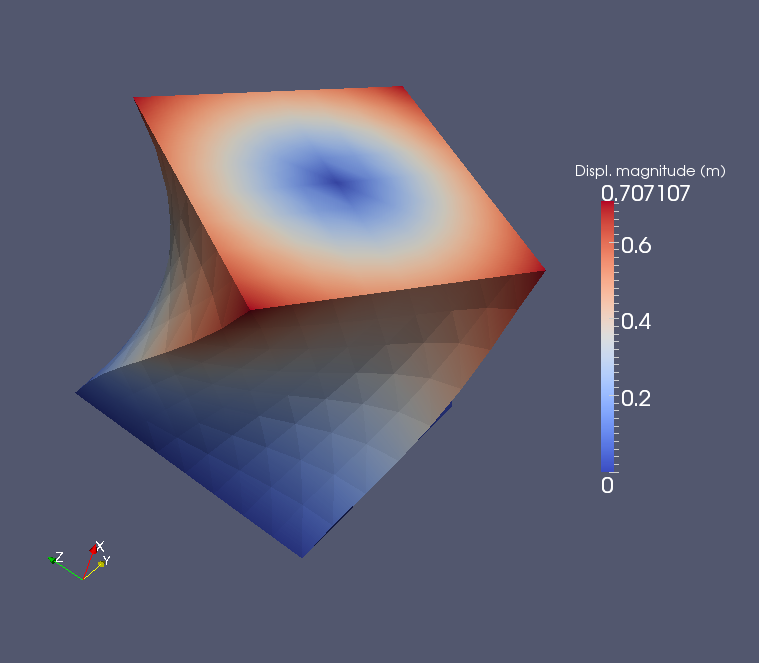
\includegraphics[width=\textwidth]{png/twistedcube.png}
    \end{column}

    \begin{column}{0.5\textwidth}
      \begin{python}
from fenics import *

mesh = UnitCubeMesh(24, 16, 16)
V = VectorFunctionSpace(mesh, "Lagrange", 1)

left =  CompiledSubDomain("(std::abs(x[0])       < DOLFIN_EPS) && on_boundary")
right = CompiledSubDomain("(std::abs(x[0] - 1.0) < DOLFIN_EPS) && on_boundary")

c = Expression(("0.0", "0.0", "0.0"), degree=0)
r = Expression(("0.0", 
"0.5*(y0+(x[1]-y0)*cos(t)-(x[2]-z0)*sin(t)-x[1])",
"0.5*(z0+(x[1]-y0)*sin(t)+(x[2]-z0)*cos(t)-x[2])"),
y0=0.5, z0=0.5, t=pi/3, degree=3)
bcl = DirichletBC(V, c, left)
bcr = DirichletBC(V, r, right)
bcs = [bcl, bcr]
v  = TestFunction(V)
u  = Function(V) 
B  = Constant((0.0, -0.5, 0.0))
T  = Constant((0.1,  0.0, 0.0))
I = Identity(V.cell().d)
F = I + grad(u)
Ic = tr(F.T*F)
J  = det(F)
E, nu = 10.0, 0.3
mu, lmbda = Constant(E/(2*(1 + nu))), Constant(E*nu/((1 + nu)*(1 - 2*nu)))
psi = (mu/2)*(Ic - 3) - mu*ln(J) + (lmbda/2)*(ln(J))**2
Pi = psi*dx - dot(B, u)*dx - dot(T, u)*ds
F = derivative(Pi, u, v)

solve(F == 0, u, bcs) 
plot(u, interactive=True, mode="displacement")
      \end{python}
    \end{column}
  \end{columns}

  % Compensate for scaling
  \huge

  \reference{H. Narayanan}
            {A computational framework for nonlinear elasticity}
            {2011}

\end{frame}

\begin{frame}[fragile]
  \frametitle{Computational hemodynamics}

  \begin{center}
    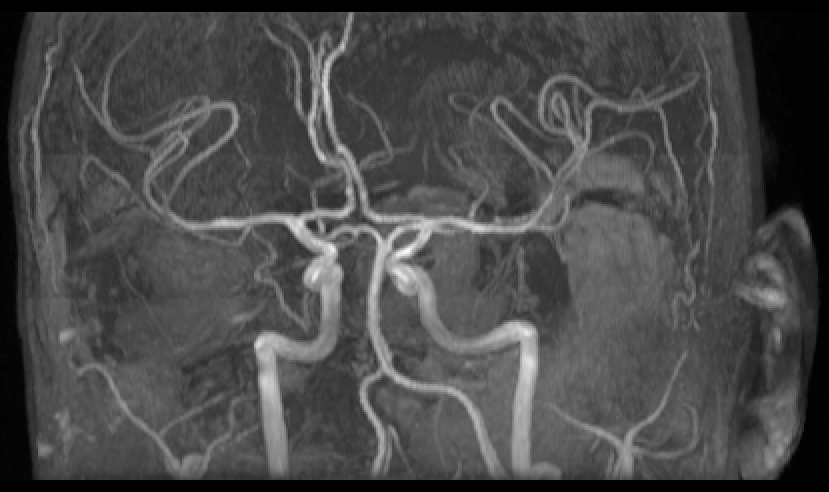
\includegraphics[height=3.5cm]{png/circle_of_willis_scan.png} \hspace{0.3cm}
    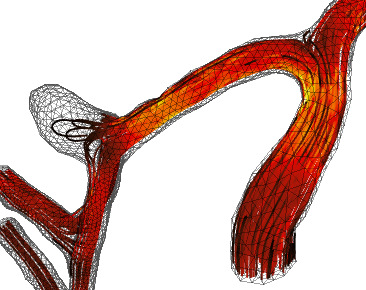
\includegraphics[height=3.5cm]{png/circle_of_willis_aneurysm.png}
  \end{center}

  \begin{itemize}
  \item
    Low wall shear stress may trigger aneurysm growth
  \item
    Solve the incompressible Navier--Stokes equations on patient-specific geometries
    \begin{displaymath}
      \begin{split}
        \dot{u} + u \cdot \nabla u - \nabla \cdot \sigma(u, p) &= f \\
        \nabla \cdot u &= 0
      \end{split}
    \end{displaymath}
  \end{itemize}

  \reference{Valen-Sendstad, Mardal, Logg}
            {Computational hemodynamics}
            {2011}

\end{frame}

\begin{frame}[fragile, shrink=50]
  \frametitle{Computational hemodynamics (contd.)}

  \vspace{2cm}

  \begin{columns}

    \begin{column}{0.5\textwidth}
      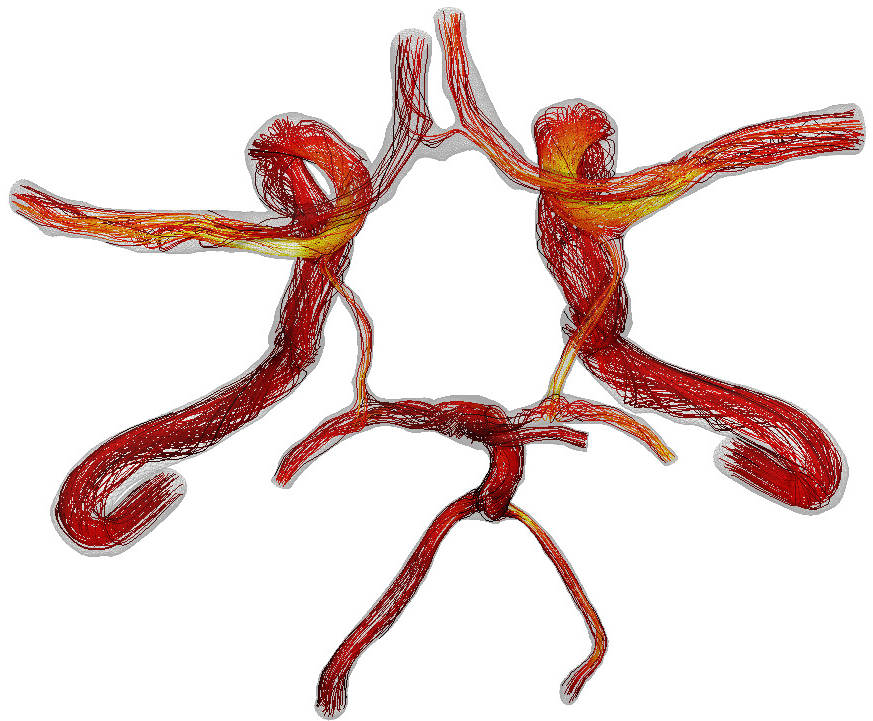
\includegraphics[width=\textwidth]{png/circle_of_willis_simulation.png}
    \end{column}

    \begin{column}{0.5\textwidth}
      \begin{python}
# Define Cauchy stress tensor
def sigma(v,w):
    return 2.0*mu*0.5*(grad(v) + grad(v).T)  - w*Identity(v.cell().d)

# Define symmetric gradient
def epsilon(v):
    return  0.5*(grad(v) + grad(v).T)

# Tentative velocity step (sigma formulation)
U = 0.5*(u0 + u)
F1 = rho*(1/k)*inner(v, u - u0)*dx + rho*inner(v, grad(u0)*(u0 - w))*dx \
   + inner(epsilon(v), sigma(U, p0))*dx \
   + inner(v, p0*n)*ds - mu*inner(grad(U).T*n, v)*ds \
   - inner(v, f)*dx
a1 = lhs(F1)
L1 = rhs(F1)

# Pressure correction
a2 = inner(grad(q), k*grad(p))*dx
L2 = inner(grad(q), k*grad(p0))*dx - q*div(u1)*dx

# Velocity correction
a3 = inner(v, u)*dx
L3 = inner(v, u1)*dx + inner(v, k*grad(p0 - p1))*dx
      \end{python}
    \end{column}

  \end{columns}

  % Compensate for scaling
  \huge

  \vspace{0.5cm}

  \begin{itemize}
  \item
    The Navier--Stokes solver is implemented in Python/FEniCS
  \item
    FEniCS allows solvers to be implemented in a minimal amount of code
  \end{itemize}

  \reference{Valen-Sendstad, Mardal, Logg}
            {Computational hemodynamics}
            {2011}

\end{frame}

\begin{frame}[fragile]
  \frametitle{Numerical relativity}

  \[ R_{ab} - \frac{1}{2} R g_{ab} + g_{ab} \Lambda = 8 \pi T_{ab} \]

  \begin{center}
    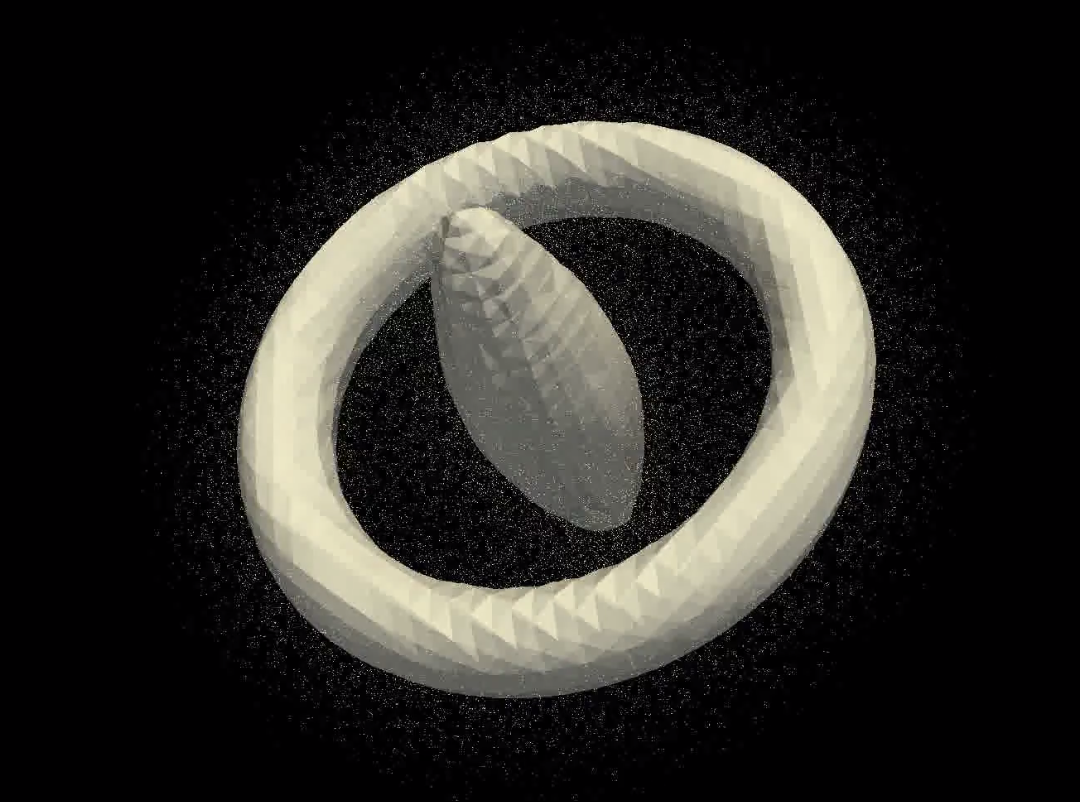
\includegraphics[width=0.8\textwidth]{png/einstein_vlasov.png}
  \end{center}


  \reference{Ames, Andreasson, Logg}
            {}
            {2015}

\end{frame}


% Show a simple taster
\begin{frame}
  \frametitle{Hello World in FEniCS: problem formulation}

  \begin{block}{Poisson's equation}
    \vspace{-0.5cm}
    \begin{displaymath}
      \begin{split}
        -\Delta u &= f \quad \mbox{ in } \Omega \\
        u &= 0 \quad \mbox { on } \partial\Omega
      \end{split}
    \end{displaymath}
  \end{block}

  \begin{block}{Finite element formulation}
    \vspace{1ex}
    Find $u \in V$ such that
    \begin{displaymath}
      \underbrace{\int_{\Omega} \nabla u \cdot \nabla v \dx}_{\textcolor{fenicsred}{a(u,v)}}
      = \underbrace{\int_{\Omega} f \, v \dx}_{\textcolor{fenicsred}{L(v)}}
      \quad \foralls v \in V
    \end{displaymath}
  \end{block}

\end{frame}

\begin{frame}[fragile]
  \frametitle{Hello World in FEniCS: implementation}

    \begin{python}
from fenics import *

mesh = UnitSquareMesh(32, 32)

V = FunctionSpace(mesh, "Lagrange", 1)
u = TrialFunction(V)
v = TestFunction(V)
f = Expression("x[0]*x[1]", degree=2)

a = dot(grad(u), grad(v))*dx
L = f*v*dx

bc = DirichletBC(V, 0.0, DomainBoundary())

u = Function(V)
solve(a == L, u, bc)
plot(u)
    \end{python}

\end{frame}

\begin{frame}
  \frametitle{Basic API}

  \begin{itemize}
  \item
    \texttt{Mesh},
    \texttt{Vertex},
    \texttt{Edge},
    \texttt{Face},
    \texttt{Facet},
    \texttt{Cell}
  \item
    \texttt{FiniteElement}, \texttt{FunctionSpace}
  \item
    \texttt{TrialFunction},
    \texttt{TestFunction},
    \texttt{Function}
  \item
    \texttt{grad()}, \texttt{curl()}, \texttt{div()}, \ldots
  \item
    \texttt{Matrix}, \texttt{Vector}, \texttt{KrylovSolver}, \texttt{LUSolver}
  \item
    \texttt{assemble()}, \texttt{solve()}, \texttt{plot()}
  \end{itemize}

  \vspace{1cm}

  \begin{itemize}
  \item
    Python interface generated semi-automatically by SWIG
  \item
    C++ and Python interfaces almost identical
  \end{itemize}

\end{frame}


% Learning more than what this course covers
\begin{frame}
    \frametitle{Sounds great, but how do I find my way through the
    jungle?}
    \begin{center}
        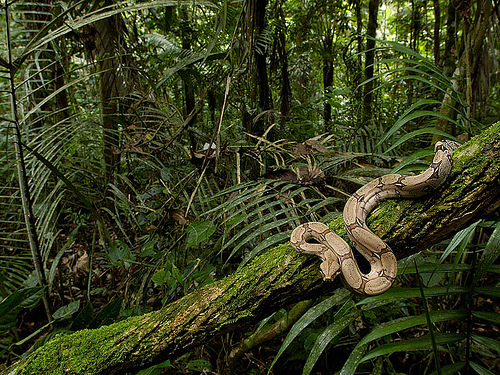
\includegraphics[width=0.8\textwidth]{jpg/jungle10.jpg}
    \end{center}
\end{frame}

\begin{frame}
    \frametitle{Three survival advices}
    \begin{columns}[c]
        \begin{column}{0.33\textwidth}
            \begin{center}
                
\includegraphics[width=0.99\textwidth]{png/python_logo.png}
            \end{center}
        \end{column}
        \begin{column}{0.33\textwidth}
            \begin{center}
                
\includegraphics[width=0.99\textwidth]{jpg/documentation.jpg}\\
            \end{center}
        \end{column}
        \begin{column}{0.33\textwidth}
            \begin{center}
                
\includegraphics[width=0.99\textwidth]{jpg/question-blue.jpg}
            \end{center}
        \end{column}
    \end{columns}
    \begin{columns}[t]
        \begin{column}{0.33\textwidth}
            \begin{center}
                \colemph{Use the right Python tools}
            \end{center}
        \end{column}
        \begin{column}{0.33\textwidth}
            \begin{center}
                \colemph{Explore the documentation}
            \end{center}
        \end{column}
        \begin{column}{0.33\textwidth}
            \begin{center}
                \colemph{Ask, report and request}
            \end{center}
        \end{column}
    \end{columns}
\end{frame}


% TODO: Update webpage images when readthedocs work is completed

% Demos on old page
\begin{frame}
  \begin{center}
     {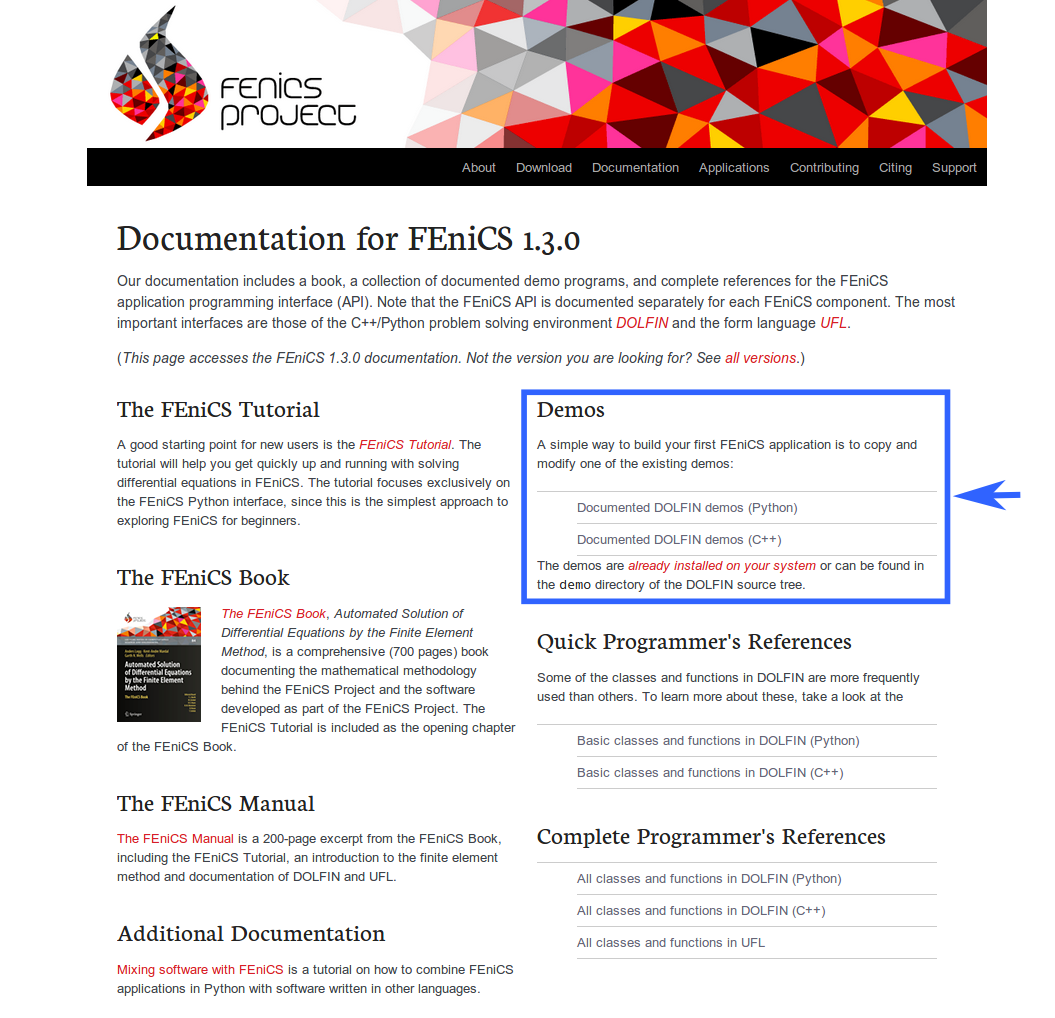
\includegraphics[width=0.80\textwidth]{png/fenics-doc-webpage-5.png}}
    \small
    \colemph{\url{http://fenicsproject.org/documentation/}}
  \end{center}
\end{frame}

% Reference docs on old page
\begin{frame}
  \begin{center}
     {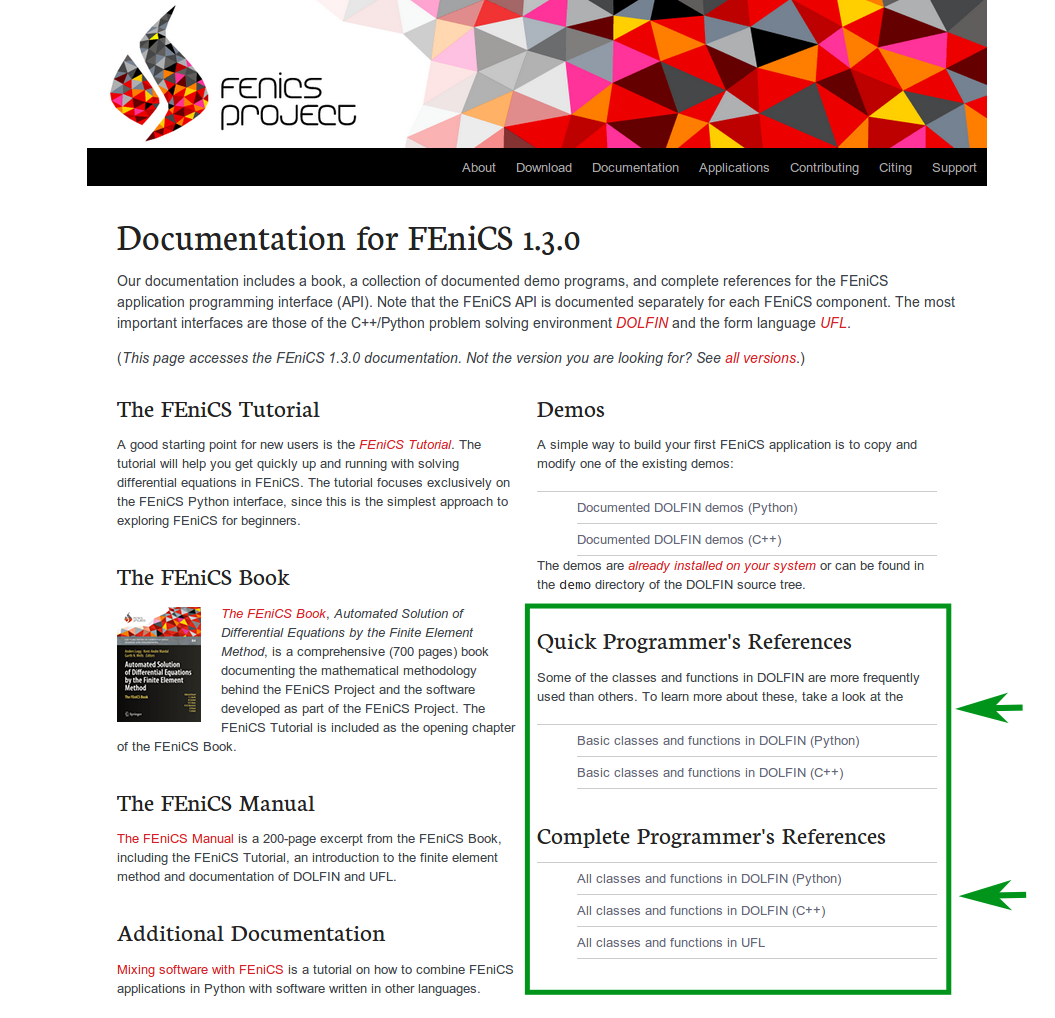
\includegraphics[width=0.80\textwidth]{png/fenics-doc-webpage-6.png}}
    \small
    \colemph{\url{http://fenicsproject.org/documentation/}}
  \end{center}
\end{frame}

% Currently migrating
\begin{frame}
  \begin{center}
     {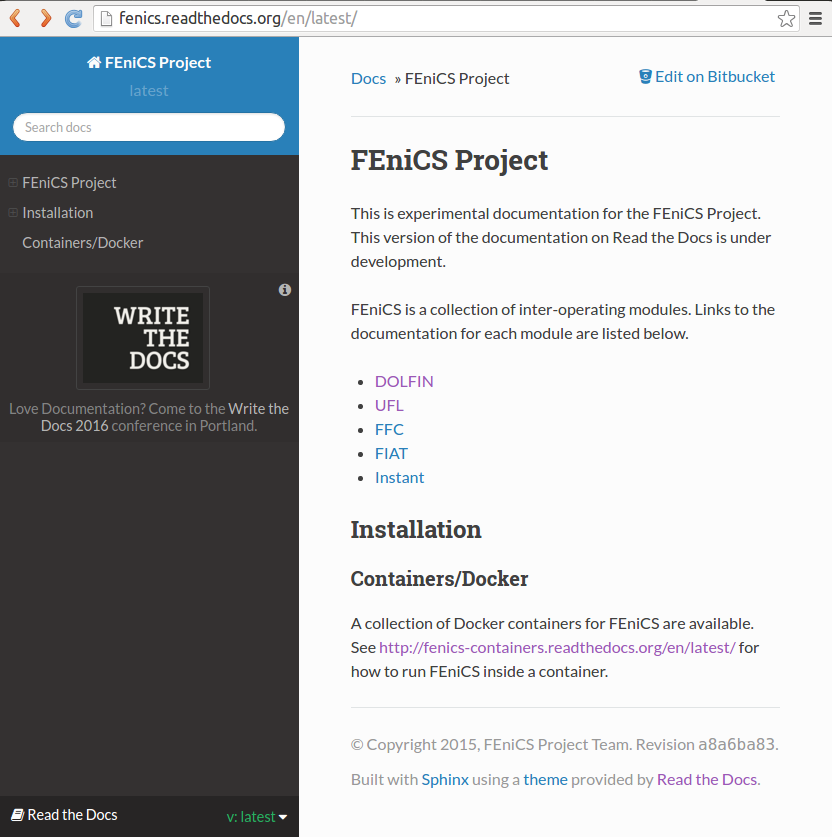
\includegraphics[width=0.80\textwidth]{png/fenics-readthedocs-webpage-1.png}}
    \small
    \colemph{\url{http://fenics.readthedocs.org/}}
  \end{center}
\end{frame}

\begin{frame}
    \frametitle{Development community is organized via bitbucket.org}
    \begin{center}
        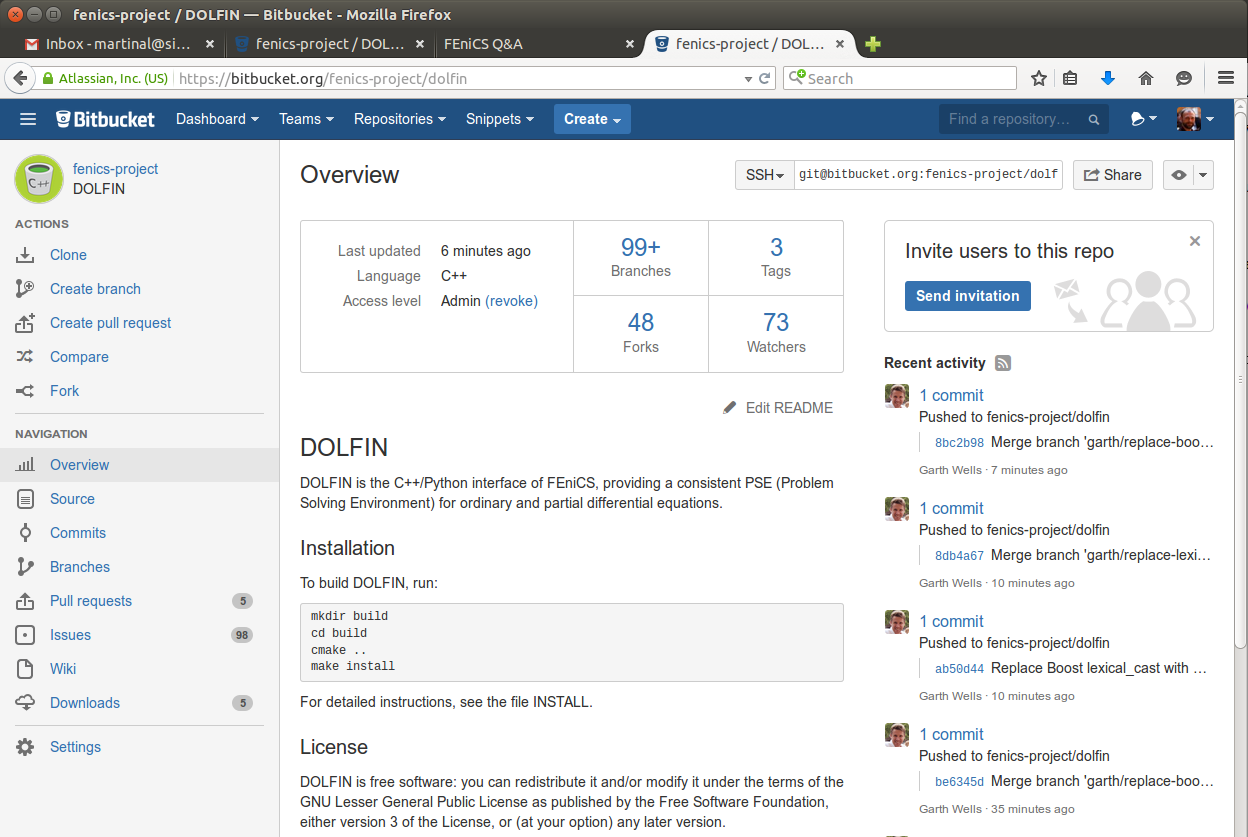
\includegraphics[height=0.75\textheight]{png/fenics-bitbucket-webpage.png}
        \vspace{1em}
        \small
        \colemph{\url{http://bitbucket.org/fenics-project/}}
    \end{center}
\end{frame}
\begin{frame}
    \frametitle{Community help is available via QA forum}
    \begin{center}
        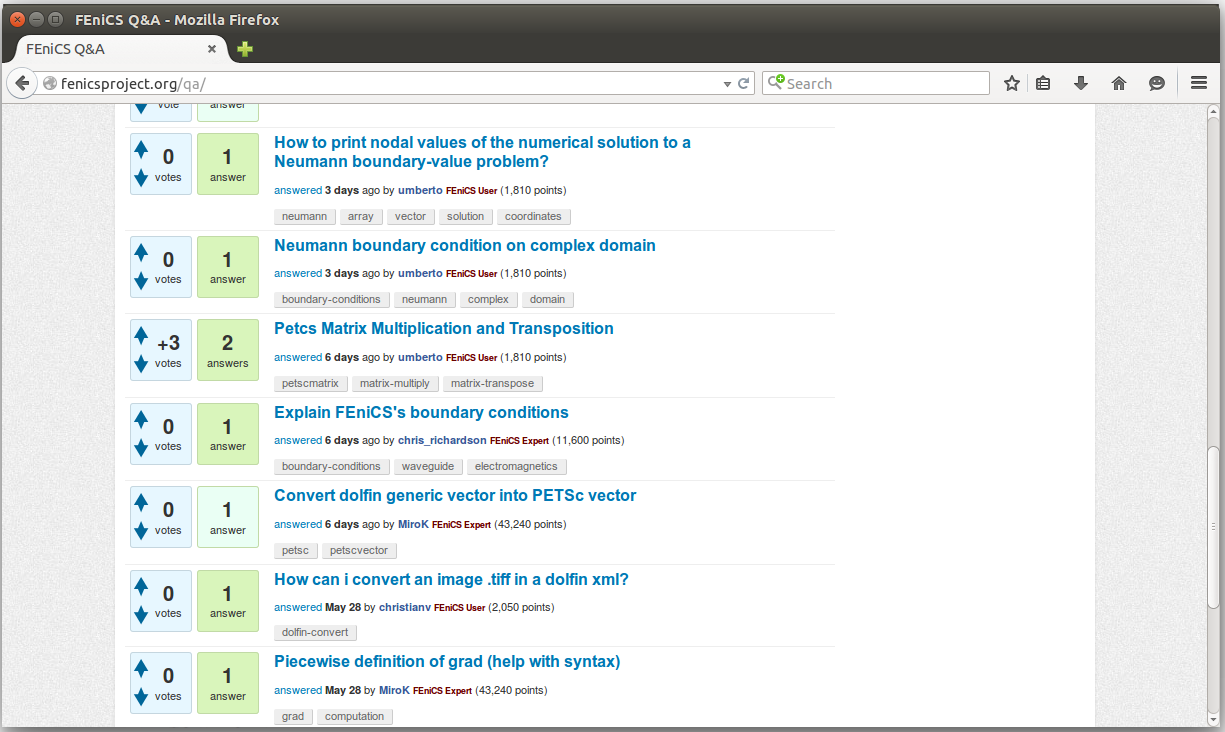
\includegraphics[width=1.0\textwidth,height=0.7\textheight]{png/fenics-qa-website.png}
        \vspace{1em}
        \small
        \colemph{\url{https://fenicsproject.org/qa}}
    \end{center}
\end{frame}


% Removed since we have a special lecture just for this
%\begin{frame}
  \frametitle{Installation alternatives}

  % FEniCS uses standard setup.py and cmake tools
  % but dependencies are tricky to configure.

  \begin{tabular}{cp{10cm}}
    
\includegraphics[height=1cm]{png/docker_logo.png} &
    \begin{minipage}{10cm}
      \ding{43} Docker images on Linux, Mac, Windows
      \vspace{0.6cm}
    \end{minipage}
    \\
    
\includegraphics[height=1cm]{png/source.png} &
    \begin{minipage}{10cm}
      \ding{43} Build from source with Hashdist (fenics-install.sh)
      \vspace{0.8cm}
    \end{minipage}
    \\
    
\includegraphics[height=1cm]{png/ubuntu_logo.png} &
    \begin{minipage}{10cm}
      \ding{43} PPA with apt packages for Debian and Ubuntu
      \vspace{0.6cm}
    \end{minipage}
    \\
    
\includegraphics[height=1cm]{png/mac_osx_logo.png} &
    \begin{minipage}{10cm}
      \ding{43} Drag and drop installation on Mac OS X
      \vspace{0.8cm}
    \end{minipage}
  \end{tabular}

  \begin{center}
    \colemph{\url{http://fenicsproject.org/download/}}
  \end{center}

\end{frame}


\begin{frame}{Let's get started and remember:}

\linespread{2.0}
\bigskip
\begin{itemize}
\item
{\footnotesize \textbf{Lectures} can be downloaded from
  \url{http://fenicsproject.org/pub/course/lectures}}

\item
{\footnotesize \textbf{Data} for exercises can be downloaded from
  \url{http://fenicsproject.org/pub/course/data} \\
(Or copy from the .../pub/data directory on alarik)}

\item
{\footnotesize \textbf{Solutions} for exercises can be downloaded from
  \url{http://fenicsproject.org/pub/course/src} \\
(Secret password needed!)
}
\end{itemize}
\linespread{1.0}\

\end{frame}

\end{document}
